\documentclass{beamer}

\usetheme{CambridgeUS}
\usecolortheme{orchid}

\usepackage{graphicx}
\usepackage{tikz}
\usepackage{listings}
\usepackage{colortbl}
\usepackage{color}


\tikzstyle{block} = [rectangle, draw, text width=4.5em, text centered, minimum height=2em]
\lstset{basicstyle=\small\ttfamily}



\lstset{
  language=Java,
  basicstyle=\ttfamily\small,
  keywordstyle=\color{blue},
  commentstyle=\color{green!60!black},
  stringstyle=\color{red},
  showstringspaces=false,
  breaklines=true
}


\definecolor{mygray}{rgb}{0.5,0.5,0.5}
\definecolor{mygreen}{rgb}{0,0.6,0}
\definecolor{myblue}{rgb}{0,0,0.8}
\lstset{language=XML,
        morekeywords={m:GetPrice, m:StockName},
        basicstyle=\ttfamily,
        keywordstyle=\color{myblue},
        commentstyle=\color{mygreen},
        stringstyle=\color{myblue},
        numbers=left,
        numberstyle=\tiny\color{mygray},
        stepnumber=1,
        numbersep=3pt,
        backgroundcolor=\color{white},
        tabsize=1,
        showspaces=false,
        showstringspaces=false
}

% Define Protobuf language
\lstdefinelanguage{protobuf}{
  keywords={message, optional, repeated, required, returns,
  service, rpc, package, syntax, string, int32, bool},
  keywordstyle=\color{blue}\bfseries,
  ndkeywords={bool, int32, float, double, string},
  ndkeywordstyle=\color{darkgray}\bfseries,
  identifierstyle=\color{black},
  tabsize=1,
  sensitive=false,
  comment=[l]{//},
  morecomment=[s]{/*}{*/},
  commentstyle=\color{purple}\ttfamily,
  stringstyle=\color{red}\ttfamily,
  morestring=[b]",
  morestring=[b]',
}

\definecolor{codegray}{gray}{0.9}
\newcommand{\code}[1]{\colorbox{codegray}{\texttt{#1}}}


\setbeamertemplate{navigation symbols}{} % Remove navigation symbols

\title{API Design and Management}
\author{Mohamed Sweelam}
\institute{Software Engineer}
\date{}

% Add the title graphic here
\titlegraphic{
\includegraphics[width=7cm, height=3.5cm]{img/course-logo.png}}
\logo{
\includegraphics[height=1cm]{img/channel-logo-circular.png}}

\begin{document}

\begin{frame}
  \titlepage
\end{frame}

\begin{frame}{Outline}
  \tableofcontents
\end{frame}

\section{Course Objectives}
\begin{frame}
	\frametitle{Course Objectives} % Table of contents slide, comment this block out to remove it
		\begin{enumerate}
			\item<1-> Provide good Arabic content for the topic
			\item<2-> Overview of API Design and Management
			\item<3-> Role and Importance of APIs in Distributed Systems
			\item<4-> The best practices you should follow today
		\end{enumerate}
\end{frame}

\section{Understanding APIs}
\begin{frame}{Understanding APIs}
	\begin{block}{Definition \tiny{\textit{wikipedia}}}
		\small{ Application programming interface (API) is a way for two or more computer programs or components to communicate with each other. It is a type of software interface, offering a service to other pieces of software.}
	\end{block}
	
	\begin{block}{Definition \tiny{\textit{ChatGPT}}}
		\small{ API (Application Programming Interface) is a set of rules, protocols, and tools for building software applications. It specifies how software components should interact and is used to enable the integration between different software systems. }
	\end{block}
	
	\begin{alertblock}{History \tiny{\textit{wikipedia}}}
		\small{ The term "application program interface" is first recorded in a paper called Data structures and techniques for remote computer graphics in 1968. The authors use the term to describe the interaction of an application "Graphics Program" with the rest of the computer system. }
	\end{alertblock}
  
\end{frame}

\begin{frame}{Understanding APIs \small{\textit OSI Model}}
	\small {The open systems interconnection (OSI) model is a conceptual model created for Standardization which enables diverse communication systems to communicate using standard protocols.} 
	\begin{center}
    		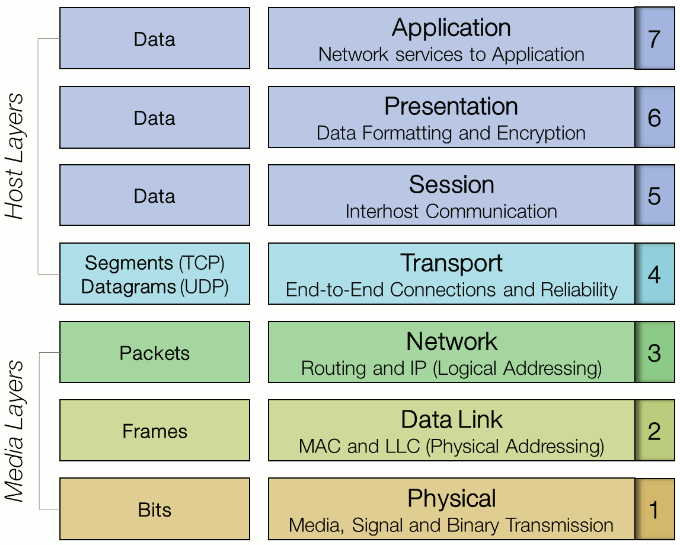
\includegraphics[width=0.8\textwidth, height=0.6\textheight]{img/osi-model.png}
  \end{center}
  \tiny { source: \href{https://www.coengoedegebure.com/osi-model}{\textcolor{blue}{coengoedegebure.com/osi-model}}}
\end{frame}

\begin{frame}{Understanding APIs \small Example}
	\begin{center}
    		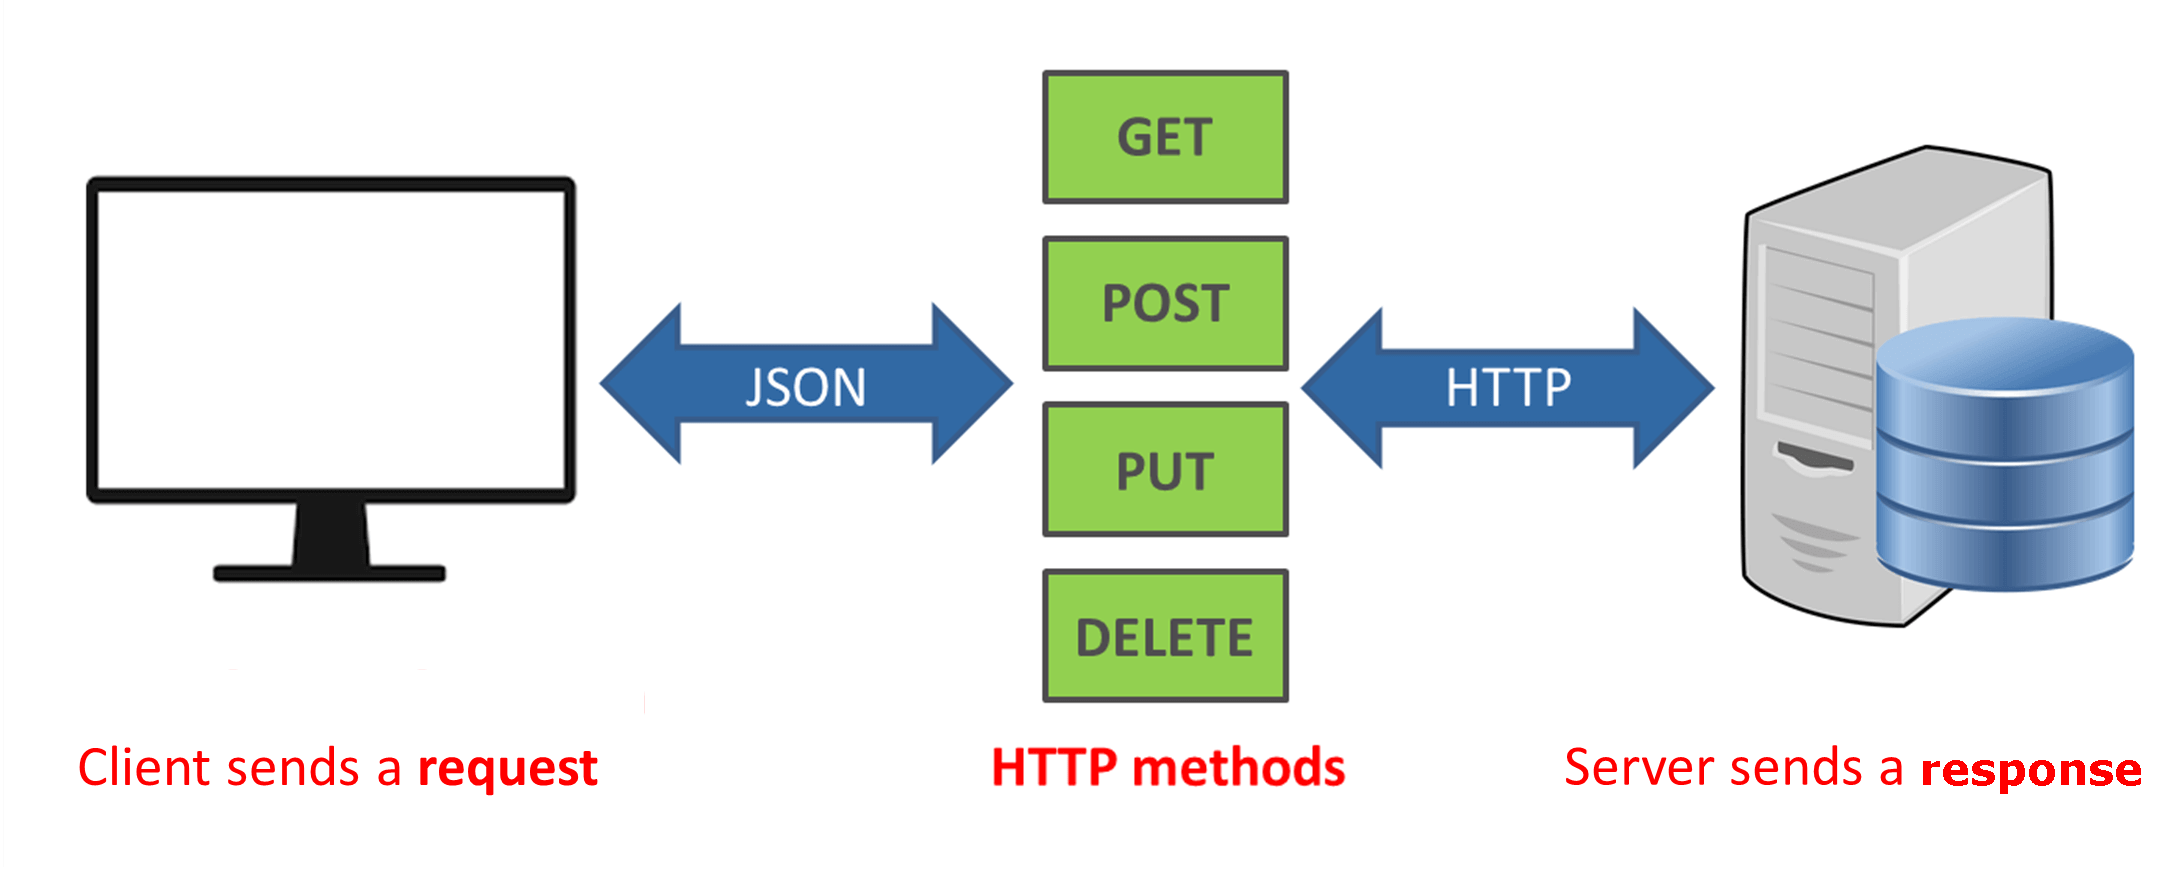
\includegraphics[width=0.6\textwidth, height=0.4\textheight]{img/api-client-to-server.png}
  \end{center}
  
  \tiny { source: \href{https://phpenthusiast.com/blog/what-is-rest-api}{\textcolor{blue}{phpenthusiast.com/blog/what-is-rest-api}}}
\end{frame}

\begin{frame}[t]{Understanding APIs \small (API Types)}
  There are several types of API, each one serves specific use case.
  
  \begin{itemize}
  	\item<1-> Public APIs (Open APIs) \\
  	\tiny{ The APIs are publicly available and can be designed in various ways, taking security into account. However, \underline{the main priority is to ensure they are easily consumable by as many clients as possible. }}

  	\item<2-> \small Partner APIs \\
  	\tiny{ Specialized interfaces that enable organizations to access data and service offerings across businesses (B2B) in order to create unique features within their own applications or services by utilizing a partner's resources. }
  	
  	\item<3-> \small Internal APIs \\
  	 \tiny{ Intended for use internally by the organizations own developers. These APIs facilitate the transmission of data between different components of a system, enabling process automation. }
  	 
  	\item<4-> \small Composite APIs  {\tiny Executes a series of API requests in a single call.}
  	\vspace{3mm}
    \item<5->[] The types can be designed and developed using two ways \\
    \begin{enumerate}
     \item API Architectural Style, 
     \item API Standard Protocol.  
    \end{enumerate}    
  \end{itemize}   
  
  
\end{frame}


\begin{frame}[t]{Understanding APIs \small (API Architecture vs API Protocols)}
  \begin{block}{API Architecture Style}  
   \scriptsize It refers to the high-level structural design of the API. It encompasses the standards, and best practices governing how the API is developed, how it interacts with other systems, and how it exposes its functionality and data.\\
   \color{teal} Example: REST
  \end{block}
  
  \begin{alertblock}{No Restrictions}
    \scriptsize Architectural style is sensitive to change and enhancement; it relies more on human experience.
  \end{alertblock}
  
  
  \begin{block}{API Protocol}
    \scriptsize It refers to a set of rules and standards used for communication between various software components. The protocol dictates how requests and responses are formatted and transmitted, and what are the restrictions of the communication.\\
    \color{teal} Example: SOAP
  \end{block}
\end{frame}

\begin{frame}[fragile,t]{Understanding APIs \small (SOAP API)}
  
  \begin{itemize}
    \scriptsize
    \item<1-> SOAP (Simple Object Access Protocol) is a protocol used for exchanging structured information in web services in computer networks. 
    \item<2-> It's a standards-based web services access protocol that has been around for a long time. 
	\item<3-> It relies on XML as its message format and usually relies on other application layer protocols, most notably Hypertext Transfer Protocol (HTTP) and Simple Mail Transfer Protocol (SMTP), for message negotiation and transmission.
	\item<4->[] 
	\tiny 
	\begin{lstlisting}
    <?xml version="1.0"?>
    <soap:Envelope xmlns:soap="http://schemas.xmlsoap.org/soap/envelope/">
      <soap:Header>
        <!-- header information here -->
      </soap:Header>
      <soap:Body>
        <m:GetPrice xmlns:m="http://www.example.org/stock">
          <m:StockName>IBM</m:StockName>
        </m:GetPrice>
      </soap:Body>
      <soap:Fault>
        <!-- fault information here -->
      </soap:Fault>
    </soap:Envelope>
    \end{lstlisting}

  \end{itemize}
  
\end{frame}

\begin{frame}[fragile,t, label=api-graphs]{Understanding APIs \small (Other Protocols)}
  
  \begin{minipage}[t]{0.2\textwidth}
    \begin{itemize}
      \item \href{https://grpc.io}{\textcolor{blue}{gRPC}}
      \item \href{https://en.wikipedia.org/wiki/REST}{\textcolor{blue}{REST}}
      \item \href{https://graphql.org}{\textcolor{blue}{GraphQL}} 
    \end{itemize}
  \end{minipage}
  \hfill
  \begin{minipage}[]{0.7\textwidth}
    \begin{center}
      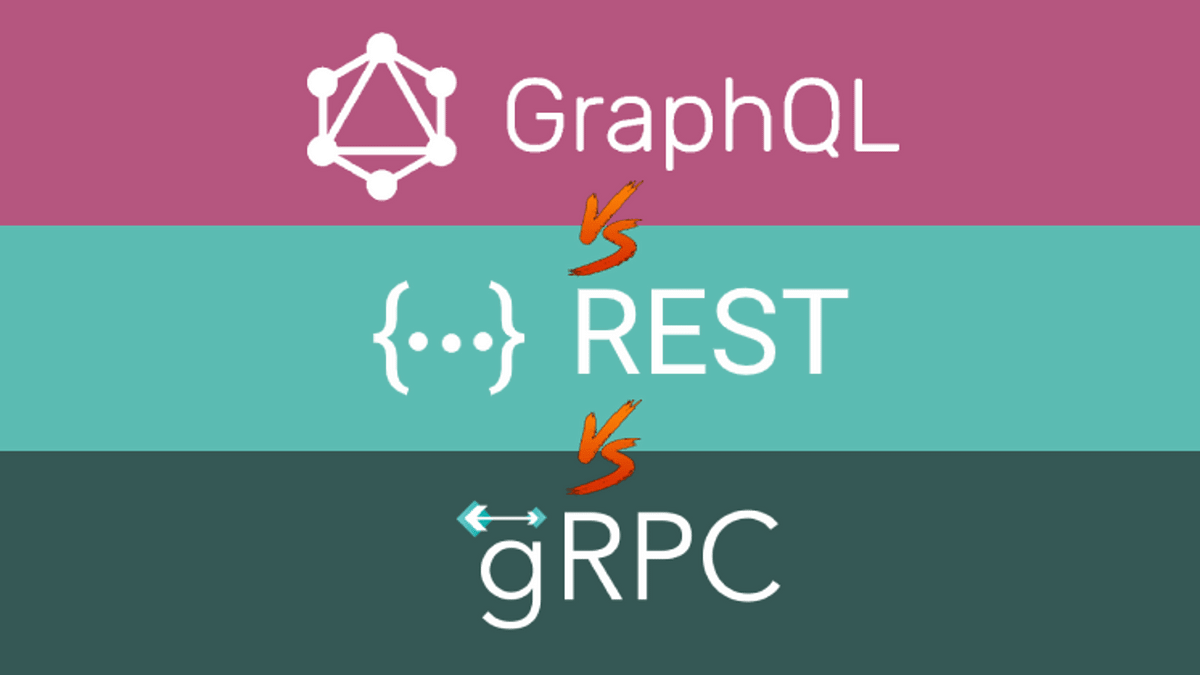
\includegraphics[width=\textwidth, height=0.6\textheight]{img/api-protocols.png}
    \end{center}
  \end{minipage}
  
  \vspace{15mm}
      \tiny { source: \href{https://mobilelive.medium.com/rest-vs-graphql-vs-grpc-comparing-three-modern-api-technologies-9ba58abadd82}{\textcolor{blue}{REST vs GraphQL vs gRPC: Comparing Three Modern API Technologies}}}

\end{frame}

\begin{frame}[fragile,t]{Understanding APIs \small (HTTP1 vs HTTP2)}  
	\begin{table}[t]
	\tiny
	\centering
		\begin{tabular}{  | >{\centering\arraybackslash}m{5cm} | >{\centering\arraybackslash}m{5cm} | }
		\hline
		\textbf{HTTP/1.1} & \textbf{HTTP/2} \\
		\hline
		Text-Based Protocol: Data is sent in a text-based format. & Binary Protocol: More efficient binary protocol, easier to parse. \\
		\hline
		One Request Per Connection: Each TCP connection allows only one request-response cycle at a time. & Multiplexing: Multiple requests and responses can be handled over a single TCP connection in parallel. \\
		\hline
		Headers Uncompressed: Headers are sent in plain text and can be quite large. & Header Compression: Uses HPACK compression to reduce overhead. \\
		\hline
		No Push Capabilities & Server Push \\
		\hline
		\end{tabular}
		\end{table}
    \begin{center}
      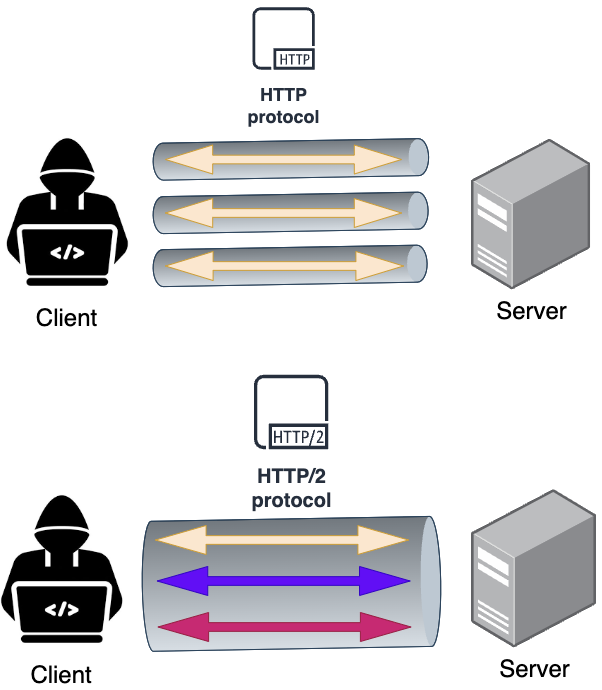
\includegraphics[width=0.6\textwidth, height=0.57\textheight]{img/http1-http2.png}
    \end{center}
  
\end{frame}

\begin{frame}[fragile,t]{Understanding APIs \small (gRPC Protocol)}  
	
	\begin{itemize}
	\scriptsize
      \item gRPC is a modern open source high performance Remote Procedure Call (RPC) framework that was developed in Google.
      \item gRPC can use \textbf{protocol buffers} as its underlying message interchange format.
      \item gRPC is based around the idea of defining a service, specifying the methods that can be called remotely with their parameters and return types.
      \tiny
      \item On the server side, the server implements this interface and runs a gRPC server to handle client calls. 
      \item On the client side, the client has a stub (referred to as just a client in some languages) that provides the same methods as the server.
    \end{itemize}
    
    \begin{center}
      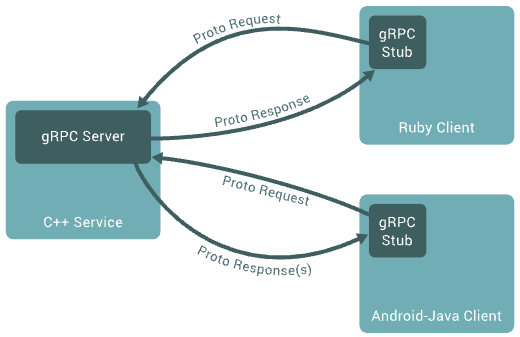
\includegraphics[width=0.5\textwidth, height=0.4\textheight]{img/grpc.png}
    \end{center}
    
    \tiny { source: \href{https://grpc.io/docs/what-is-grpc/introduction/}{\textcolor{blue}{Introduction to gRPC}}}
  
\end{frame}

\begin{frame}[fragile,t]{Understanding APIs \small (Protocol Buffers)}  
	
	\begin{itemize}
	\scriptsize
      \item Protocol Buffers are a language-neutral, platform-neutral extensible mechanism for serializing structured data.
      \item The file that includes the definition is \code {.proto} file
      
      \item[] 
      \scriptsize
      \begin{lstlisting}[language=protobuf]
		message Person {
			string name = 1;
			int32 id = 2;
			bool has_kids = 3;
			optional string email = 4;
		}
      \end{lstlisting}
    \end{itemize}
    
    \begin{center}
      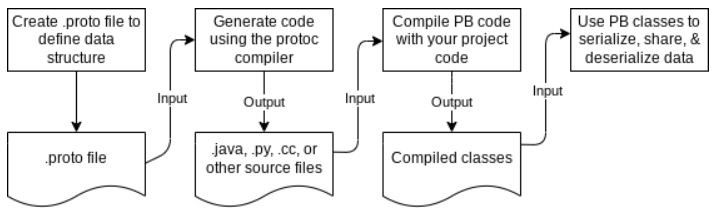
\includegraphics[width=0.7\textwidth, height=0.3\textheight]{img/protobuf-img.png}
    \end{center}
    
    \tiny { source: \href{https://protobuf.dev/overview/}{\textcolor{blue}{protobuf overview}}}
  
\end{frame}

\begin{frame}[fragile,t]{Understanding APIs \small (gRPC)}  

    \begin{center}
      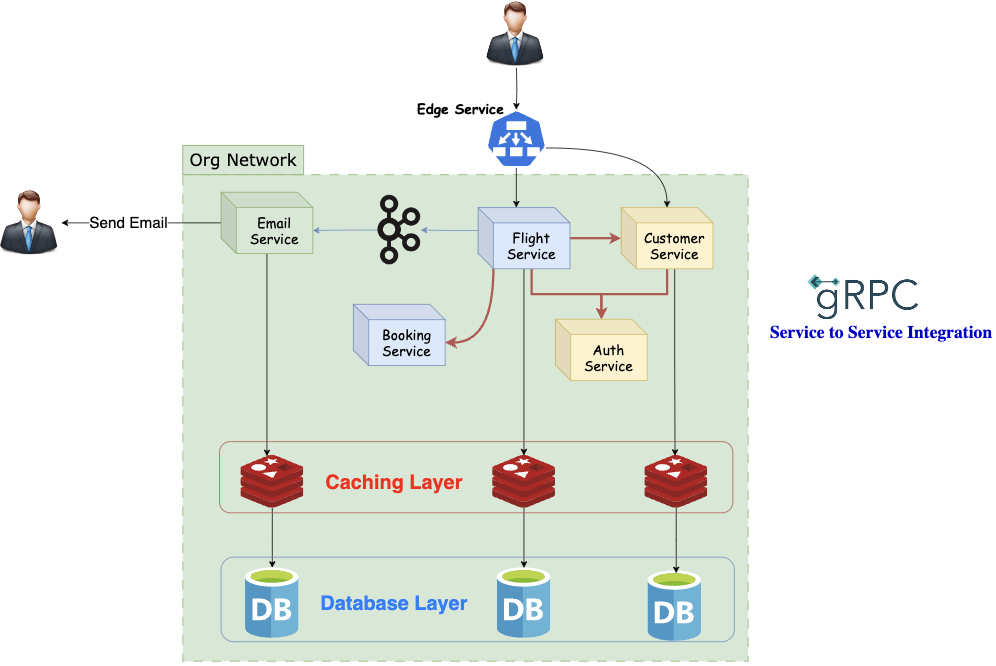
\includegraphics[width=0.8\textwidth, height=0.7\textheight]{img/flight-gRPC.png}
    \end{center}
    \tiny { source: \href{https://grpc.io/docs/what-is-grpc/introduction/}{\textcolor{blue}{gRPC Offical doc}}}
  
\end{frame}

\begin{frame}[fragile,t]{Understanding APIs \small (gRPC)}  
	
	\scriptsize
      \begin{lstlisting}[language=protobuf]
		syntax = "proto3";
		package observer;

		service ObserverStatusService {
    		rpc getServiceStatus (SystemStatusRequest) 
    				returns (SystemStatusResponse) {}
		}

		message SystemStatusRequest {
    		optional string uuid = 1;
    		string service_name = 2;
		}

		message SystemStatusResponse {
    		string uuid = 1;
    		string status = 2;
    		string component = 3;
    		optional string service_name = 4;
		}
      \end{lstlisting}
  
\end{frame}

\againframe{api-graphs}

\begin{frame}[t]{Understanding APIs \small (RESTful API)}
  
    \scriptsize 
  \begin{block}{REST API}  
   \begin{itemize}
    \scriptsize 
   	\item In 2000, Roy Fielding proposed Representational State Transfer (REST) as an architectural approach to designing web services
   	\item REST is independent of any underlying protocol and is not necessarily tied to HTTP
   	\item REST is an architectural style for building distributed systems based on \textit{hypermedia}
   \end{itemize}	   
  \end{block}  
  
    \scriptsize  
  \begin{block}{Primary Goal}  
  \scriptsize
	 {REST API doesn't bind the implementation to any specific implementation, the API could be written in \textbf{Go} , and the client can use any language or tools.}	   
  \end{block}  
  
  \scriptsize
  \begin{example}
  	  	\scriptsize To \textbf{GET} an order , API URI might look like https://api-design/orders/1 \\
  		\scriptsize Client response \code {\{"orderId":1,"orderValue":99.90,"productId":1,"quantity":1\}}
  \end{example}
  
  \tiny { source: \href{https://learn.microsoft.com/en-us/azure/architecture/best-practices/api-design}
  		{\textcolor{blue}{Microsoft: RESTful web API design}}}
  
\end{frame}

\begin{frame}[t]{Understanding APIs \small (RESTful API)}
	
	\scriptsize 
	\begin{block}{It is all about \textit{resources}}
		A resource is an entity that can be identified, named, addressed, or handled on the web.REST APIs expose data as resources
		and use standard HTTP methods to represent Create, Read, Update, and Delete (CRUD) transactions against these resources.
	\end{block}  
  
  \scriptsize 
   \begin{itemize}
    \scriptsize 
   	\item<2-> Resource is part of URL like, https://api-design/\textbf{orders}/1
   	\item<3-> Resource is always noun and plural, for each resource, two URLs are generally implemented one for collection, 
   	and one for specific element.\\ like, \textit{\textbf{/users}} and \textit{\textbf{/users/12}}
   	\item<4-> HTTP methods like GET, POST, UPDATE, and DELETE inform the server about the action to be performed
   	\item<5-> REST methods semantics ``CRUD``
   		\begin{itemize}
   			\scriptsize 
  			\item READ   \hspace{0.53cm} $\rightarrow$ GET, \texttt{never change the server state}
   			\item CREATE \hspace{0.2cm}  $\rightarrow$ POST
   			\item UPDATE \hspace{0.15cm} $\rightarrow$ PUT or PATCH
   			\item DELETE \hspace{0.18cm} $\rightarrow$ DELETE
   		\end{itemize}
   \end{itemize}	   
  
  \vspace{2mm}
  \scriptsize { source: \href{https://www.oreilly.com/library/view/designing-web-apis/9781492026914/}
  		{\textcolor{blue}{Designing Web APIs}}}
  
\end{frame}

\begin{frame}[t, label=crud-ops]{Understanding APIs \small (RESTful API)}
	
	\center \scriptsize \texttt{CRUD operations, HTTP verbs, and REST conventions}
	\begin{center}
      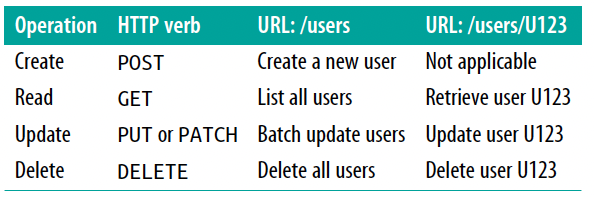
\includegraphics[width=0.7\textwidth, height=0.4\textheight]{img/crud.png}
    \end{center}
  
  \vspace{10mm}
  \tiny { source: \href{https://www.oreilly.com/library/view/designing-web-apis/9781492026914/}
  		{\textcolor{blue}{Designing Web APIs}}}
  
\end{frame}

\againframe{api-graphs}

\begin{frame}[t]{Understanding APIs \small (Intro to GraphQL)}
	\begin{block}{What is GraphQL?}
	\scriptsize
		\begin{itemize}
			\item<1-> As shown in the name, it includes ``Graph`` which means it represents a relation to some extend, you have to keep in your mind this subtle notice.
			\item<2-> GraphQL is a query language for your API, and a server-side runtime for executing queries using a type system you define for your data. 
			\item<3-> GraphQL \textbf{isn't tied} to any specific database or storage engine and is instead backed by your existing code and data.		
		\end{itemize}
	\end{block}
	
	\vspace{40mm}
	\tiny { source: \href{https://graphql.org/learn/}{\textcolor{blue}{Introduction to GraphQL}}}
\end{frame}

\begin{frame}[t]{Understanding APIs \small (Intro to GraphQL)}
	\begin{block}{What is GraphQL?}
	\scriptsize
		\begin{itemize}
			\item<1> As shown in the name, it includes ``Graph`` which means it represents a relation to some extend, you have to keep in your mind this subtle notice.
			\item<1> GraphQL is a query language for your API, and a server-side runtime for executing queries using a type system you define for your data. 
			\item<1> GraphQL \textbf{isn't tied} to any specific database or storage engine and is instead backed by your existing code and data.		
		\end{itemize}
	\end{block}
	

	\begin{example}
		\tiny
		A GraphQL service is created by defining types and fields on those types, then providing functions for each field on each type. For example, a GraphQL service that tells you who the logged in user is (me) as well as that user's name might look like this:
	\end{example}
	\begin{center}
   		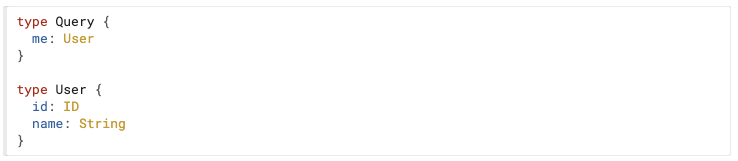
\includegraphics[width=0.7\textwidth, height=0.25\textheight]{img/graphql-example.png}
    \end{center}
    
    \tiny { source: \href{https://graphql.org/learn/}{\textcolor{blue}{Introduction to GraphQL}}}
  
\end{frame}

\begin{frame}[t]{Understanding APIs \small (Intro to GraphQL ``examples``)}
\center
	\begin{center}
   		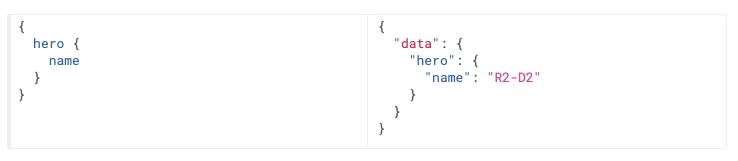
\includegraphics[width=0.5\textwidth, height=0.25\textheight]{img/graphql-example-2.png}
    \end{center}
    
    \begin{center}
   		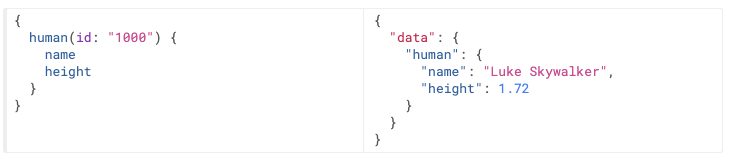
\includegraphics[width=0.5\textwidth, height=0.25\textheight]{img/graphql-example-3.png}
    \end{center}
    
    \tiny { source: \href{https://graphql.org/learn/}{\textcolor{blue}{Introduction to GraphQL}}}
\end{frame}


\begin{frame}[t]{Understanding APIs \small (Websockets API)}

\begin{block}{What is Websocket API?}
		\begin{itemize}
		\scriptsize
			\item<1-> The WebSocket API is an advanced technology that makes it possible to open a two-way interactive communication session between the user's browser and a server.
			\item<2->  With this API, you can send messages to a server and receive event-driven responses without having to poll the server for a reply.
		\end{itemize}
	\end{block}
    
    \begin{center}
   		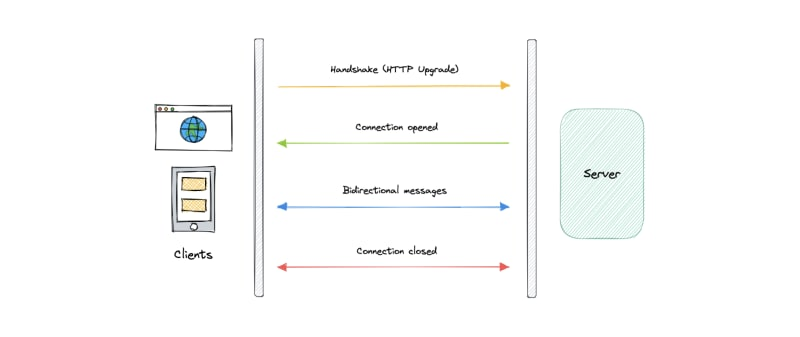
\includegraphics[width=0.8\textwidth, height=0.5\textheight]{img/websockets.jpeg}
    \end{center}
    
    \tiny { source: \href{https://dev.to/karanpratapsingh/system-design-long-polling-websockets-server-sent-events-sse-1hip}{\textcolor{blue}{WebSockets, Long polling, Server-Sent Events}}}
\end{frame}

\begin{frame}[t]{Understanding APIs}
\center
	\begin{center}
   		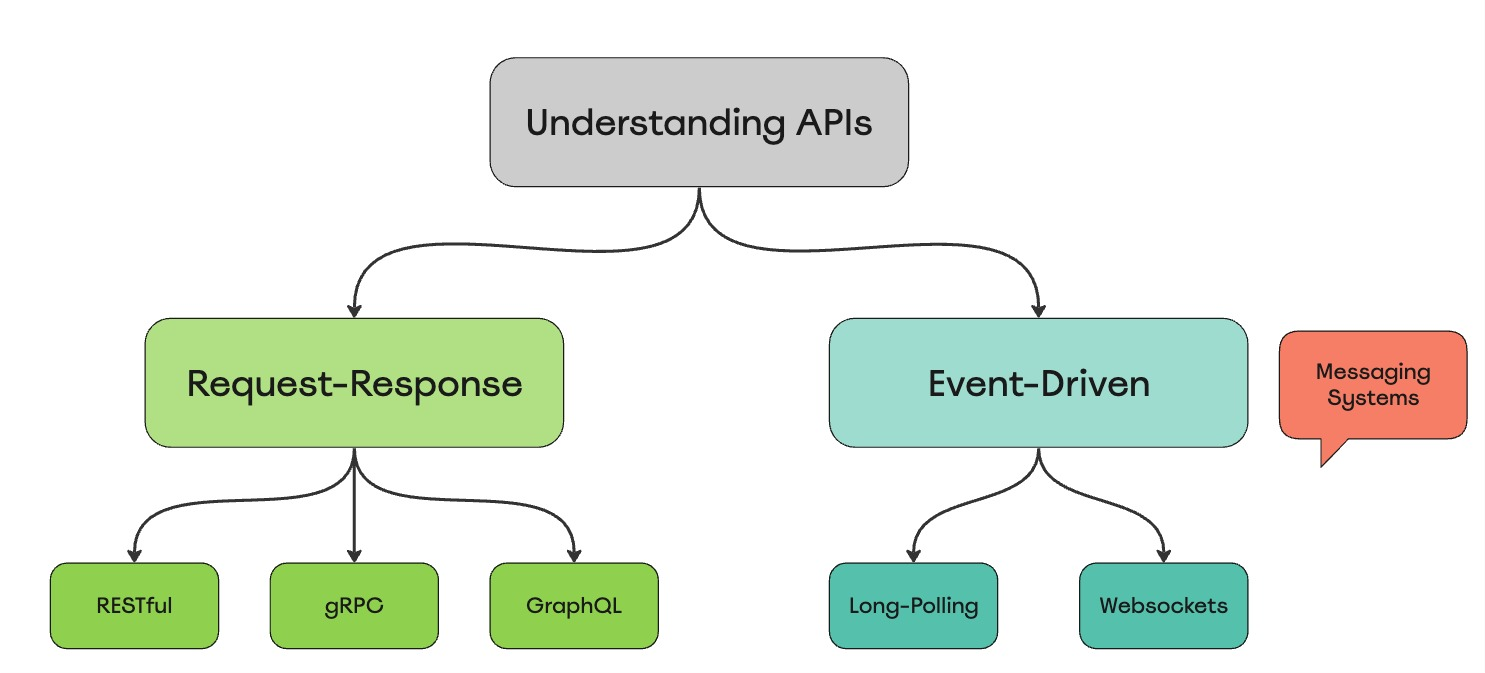
\includegraphics[width=0.8\textwidth, height=0.7\textheight]{img/understanding-apis.jpg}
    \end{center}
\end{frame}


\section{API Design Principles}
\begin{frame}{API Design Principles (Know Your Consumer)}
		\scriptsize
  When designing an API, it's best to consider real-life use cases and think about the developers who will be using your API
  \begin{itemize}
  
    \item<1-> What tasks should they be able to complete with your API? 
    \item<2-> What kind of application should developer be able to build?
    \item<3-> How can you make the developer understand your API clearly?
    \item<4->[] 
    	\begin{block}{Think Twice when Designing an API}
			 API you design is like a window that shows what you want outsiders to see.
		\end{block}
	\item<5->[]
		\begin{center}
   			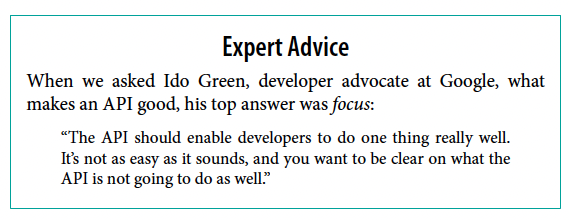
\includegraphics[width=0.6\textwidth, height=0.4\textheight]{img/advice-API.png}
	    \end{center}
    
  \end{itemize}
  
  \tiny { source: \href{https://www.oreilly.com/library/view/designing-web-apis/9781492026914/}{\textcolor{blue}{Designing Web APIs}}}
\end{frame}

\begin{frame}{API Design Principles (Best Practices)}
	\scriptsize
	Think of your API as the UI you provide to someone, check the UX multiple times. 
  \begin{itemize}
    \item<2-> Make it fast and Easy to Get Started
    \item<3-> Documentation that outline the specifications of an API can go a long way toward helping developers get started
    	\begin{itemize}
    		\scriptsize
		    \item<4-> A tutorial is an interactive interface to teach developers about your API
		    \item<5-> A guide is a more contextual document than a specification. It provides information for developers at a certain point in time—typically when getting started
	    \end{itemize}
    \item<6->[]
    	\begin{center}
   			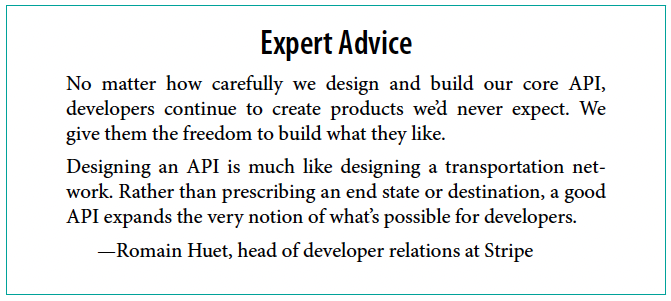
\includegraphics[width=0.6\textwidth, height=0.3\textheight]{img/advice-api-2.png}
	    \end{center}
  \end{itemize}
    
  \tiny { source: \href{https://www.oreilly.com/library/view/designing-web-apis/9781492026914/}{\textcolor{blue}{Designing Web APIs}}}
\end{frame}

\begin{frame}{API Design Principles (Request Packets)}
	\scriptsize
	HTTP Protocol was built on top of TCP protocol
	\begin{itemize}
    \item HTTP Request is sent to server over TCP IP PACKET
    \item Server Reply with ACK , PSH, and provide Response in another IP PACKET
    \item CLIENT can follow up with ACK and close the connection
  \end{itemize}
  
   	\begin{center}
   		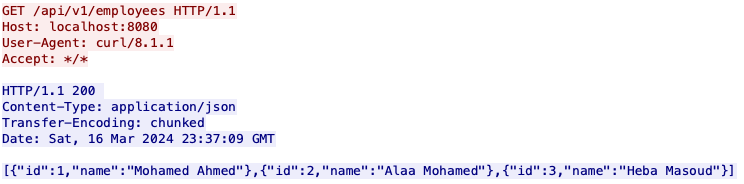
\includegraphics[width=0.6\textwidth, height=0.4\textheight]{img/api-request-details.png}
	\end{center}
    
\end{frame}

\begin{frame}{API Design Principles (Request Packets)}
	\scriptsize
	HTTP Protocol was built on top of TCP protocol
	\begin{itemize}
    	\item HTTP Request is sent to server over TCP IP PACKET
    	\item Server Reply with ACK , PSH, and provide Response in another IP PACKET
    	\item CLIENT can follow up with ACK and close the connection
  	\end{itemize}  
   	\begin{center}
   		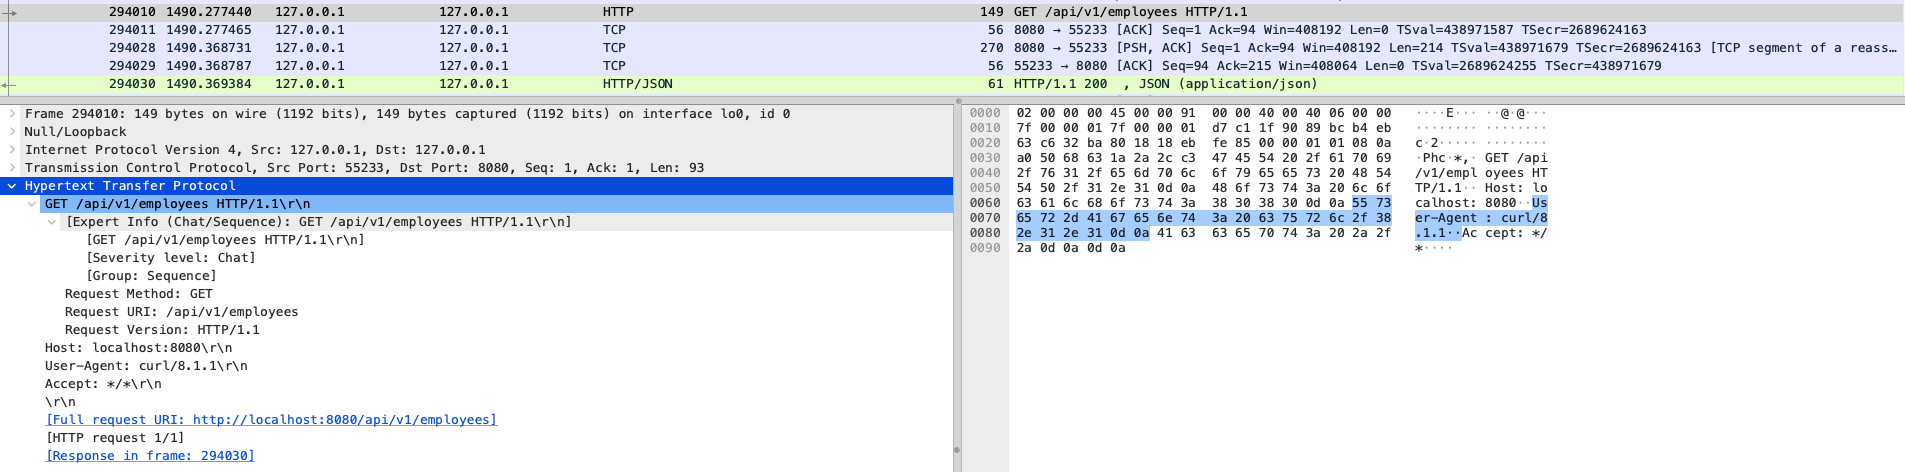
\includegraphics[width=0.8\textwidth, height=0.5\textheight]{img/api-request.png}
	\end{center}
    
\end{frame}

\begin{frame}{API Design Principles (Request Packets)}
	\scriptsize
	HTTP Protocol was built on top of TCP protocol
	\begin{itemize}
    	\item HTTP Request is sent to server over TCP IP PACKET
    	\item Server Reply with ACK , PSH, and provide Response in another IP PACKET
    	\item CLIENT can follow up with ACK and close the connection
  	\end{itemize}  
  	
   	\begin{center}
   		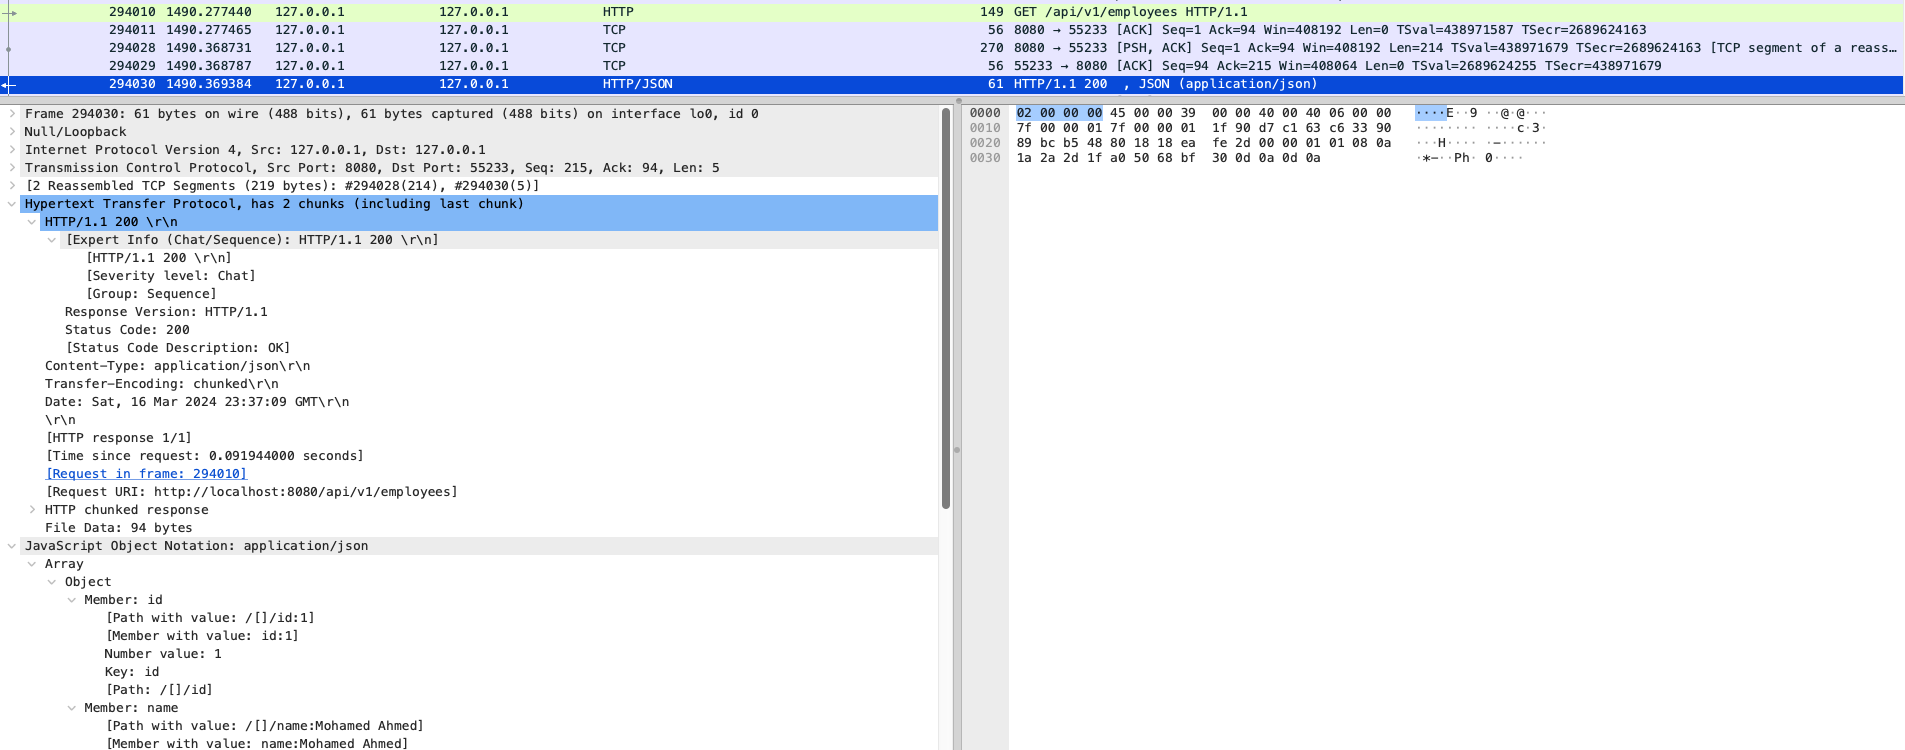
\includegraphics[width=0.8\textwidth, height=0.5\textheight]{img/api-response.png}
	\end{center}
    
\end{frame}

\section{RESTful API Design}
\begin{frame}{RESTful API Design}
  \begin{itemize}
    \item RESTful Architecture Principles
    \item Designing RESTful Services (HTTP Methods, Status Codes)
    \item Best Practices in RESTful API
  \end{itemize}
\end{frame}


\begin{frame}[t]{RESTful Architecture Principles}
	\scriptsize
	In late 1993, Roy Fielding, co-founder of the Apache HTTP Server Project recognized that the Web’s scalability was governed by a set of key constraints which were grouped under six categories:
	\begin{itemize}
    	\item \textcolor{teal}{Client-server}
    	\item \textcolor{teal}{Uniform interface}
    	\item Layered system
    	\item Stateless
    	\item Code-on-demand `Optional`
    	\item \textcolor{red} {Cache}
	\end{itemize}
\end{frame}

\begin{frame}[t]{RESTful Architecture Principles}
	\scriptsize
	In late 1993, Roy Fielding, co-founder of the Apache HTTP Server Project recognized that the Web’s scalability was governed by a set of key constraints which were grouped under six categories:
	\begin{itemize}
    	\item \textcolor{teal}{Client-server}
    	\item \textcolor{teal}{Uniform interface}

    	\item Layered system
    	\item[] \textcolor{gray}{\tiny The layered system constraints enable network-based intermediaries such as proxies and gateways to be transparently deployed between a client and server using the Web’s uniform interface.} 
    	
    	\item Stateless
    	\item Code-on-demand `Optional`
    	\item \textcolor{red} {Cache}
	\end{itemize}
\end{frame}


\begin{frame}[t]{RESTful Architecture Principles}
	\scriptsize
	In late 1993, Roy Fielding, co-founder of the Apache HTTP Server Project recognized that the Web’s scalability was governed by a set of key constraints which were grouped under six categories:
	\begin{itemize}
    	\item \textcolor{teal}{Client-server}
    	\item \textcolor{teal}{Uniform interface}

    	\item Layered system
    	\item[] \textcolor{gray}{\tiny The layered system constraints enable network-based intermediaries such as proxies and gateways to be transparently deployed between a client and server using the Web’s uniform interface.} 
    	
    	\item Stateless
    	\item[] \textcolor{gray}{ \tiny The stateless constraint dictates that a web server is not required to memorize the state of its client applications. As a result, each client must include all of the contextual information that it considers relevant in each interaction with the web server. }
    	
    	\item Code-on-demand `Optional`
    	\item \textcolor{red} {Cache}
	\end{itemize}
\end{frame}


\begin{frame}[t]{RESTful Architecture Principles}
	\scriptsize
	In late 1993, Roy Fielding, co-founder of the Apache HTTP Server Project recognized that the Web’s scalability was governed by a set of key constraints which were grouped under six categories:
	\begin{itemize}
    	\item \textcolor{teal}{Client-server}
    	\item \textcolor{teal}{Uniform interface}

    	\item Layered system
    	
    	\item[] \textcolor{gray}{\tiny The layered system constraints enable network-based intermediaries such as proxies and gateways to be transparently deployed between a client and server using the Web’s uniform interface.} 
    	
    	\item Stateless
    	\item[] \textcolor{gray}{ \tiny The stateless constraint dictates that a web server is not required to memorize the state of its client applications. As a result, each client must include all of the contextual information that it considers relevant in each interaction with the web server. }
    	
    	\item Code-on-demand `Optional`
    	\item[] \textcolor{gray}{\tiny Code-on-demand enables web servers to temporarily transfer executable programs, such as scripts or plug-ins, to clients.}

    	\item \textcolor{red} {Cache}
	\end{itemize}
\end{frame}

\begin{frame}[t]{Restful API Design Semantics}
	\scriptsize
	HTTP semantics include the intentions defined by each request method
	
	\begin{block}{HTTP Core Semantics}
		\begin{itemize}
			\item In request header fields, status codes that describe the response
			\item \textbf{Representation} metadata describe how content is intended to be interpreted by a recipient
			\item Request header fields that might influence content selection, and the various selection algorithms that are collectively referred to as "content negotiation"
		\end{itemize}				
	\end{block}	
	
	\begin{block}{Representation Definition}
		A "representation" is information that is intended to reflect a past, current, or desired state of a given resource. A representation consists of a set of representation metadata and a potentially unbounded stream of representation data.
	\end{block}		
		
	\begin{center}
   		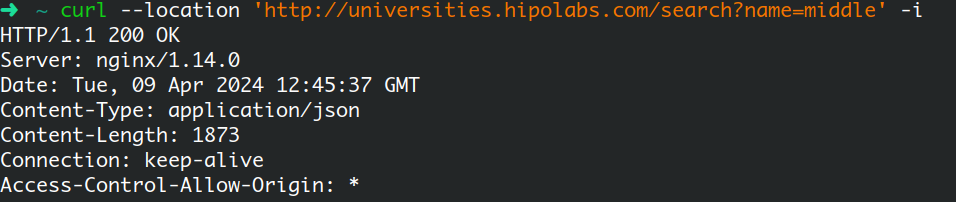
\includegraphics[width=0.6\textwidth, height=0.2\textheight]{img/header-metadata.png}
	\end{center}
	
	  \tiny source: \href{https://www.rfc-editor.org/rfc/rfc9110.html} {\textcolor{blue}{RFC 9110}} 

\end{frame}


\begin{frame}[t]{Restful API Design Semantics "Content Type"}
	\scriptsize	
		\begin{itemize}
			\item Content-Type: The indicated media type defines both the data format and how that data is intended to be processed by a recipient.
			\item[] [Format]
			\item[] Content-Type: [media type];[subtype]
			\item[] \code{Content-Type: text/html ; Charset="utf-8"}   
			\begin{examples}
				application/json 				   \hfill image/png   			\\
				application/x-www-form-urlencoded  \hfill multipart/form-data   \\
			\end{examples}
			\item \alert{Understanding the Media type helps you handling the request correctly with minimal processing}
		\end{itemize}	
		
		
		\begin{center}
   			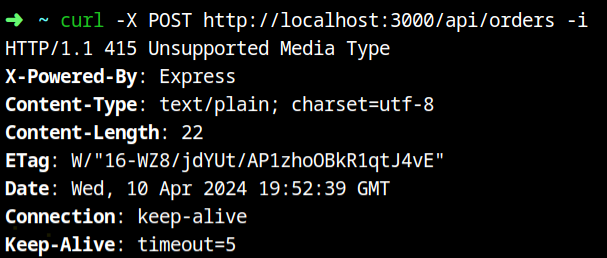
\includegraphics[width=0.6\textwidth, height=0.3\textheight]{img/unspported-media-type.png}
		\end{center}		
	
	  \tiny source: \href{https://www.rfc-editor.org/rfc/rfc9110.html} {\textcolor{blue}{RFC 9110}} 
\end{frame}

\begin{frame}[t]{Restful API Design "HTTP Methods"}
		
		\begin{center}
   			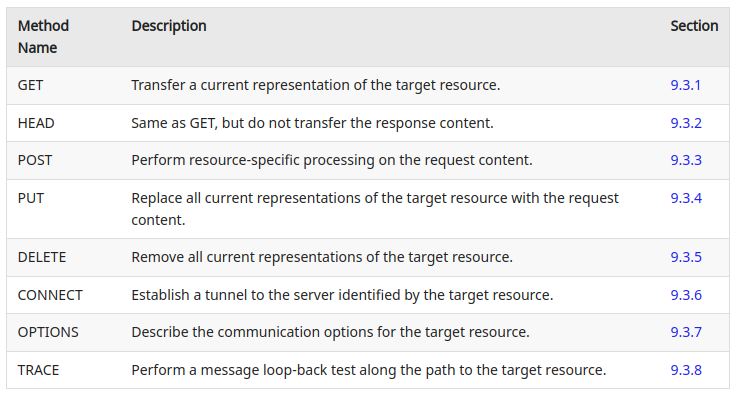
\includegraphics[width=0.8\textwidth, height=0.6\textheight]{img/http-methods.png}
		\end{center}		
	
	  \tiny source: \href{https://www.rfc-editor.org/rfc/rfc9110.html} {\textcolor{blue}{RFC 9110}} 
\end{frame}

\begin{frame}[t]{Restful API Design Semantics "Common Properties"}
	\scriptsize
	\begin{block}{Safe Methods}
		An HTTP method is safe if a request using this method doesn’t alter the state of the server. In other words, it leads to a read-only operation.\\
		\begin{itemize}
			\item Safe methods: \code{GET, HEAD, OPTIONS}
			\item Unsafe methods: \code{POST, PUT, DELETE, CONNECT, PATCH}
		\end{itemize}				
	\end{block}
	
	\vspace{44mm}
	\tiny source: \href{https://learning.mlytics.com/the-internet/http-request-methods} {\textcolor{blue}{Common Properties}} 
\end{frame}

\begin{frame}[t]{Restful API Design Semantics "Common Properties"}
	\scriptsize
	\begin{block}{Safe Methods}	
		An HTTP method is safe if a request using this method doesn’t alter the state of the server. In other words, it leads to a read-only operation.
	\end{block}
		
	\begin{block}{Idempotent Methods}
		An HTTP method is idempotent if multiple identical requests using this method will have the same effect on the server as that of a single request of that same method.\\
		\begin{itemize}
			\item Idempotent methods: \code{GET, HEAD, PUT, DELETE, OPTIONS, TRACE}
			\item Non-idempotent methods: \code{POST, CONNECT, PATCH}
		\end{itemize}	
	\end{block}
	
	\vspace{27mm}
	\tiny source: \href{https://learning.mlytics.com/the-internet/http-request-methods} {\textcolor{blue}{Common Properties}} 
\end{frame}

\begin{frame}[t]{Restful API Design Semantics "Common Properties"}
	\scriptsize
	\begin{block}{Safe Methods}		
		An HTTP method is safe if a request using this method doesn’t alter the state of the server. In other words, it leads to a read-only operation.	
	\end{block}
		
	\begin{block}{Idempotent Methods}	
		An HTTP method is idempotent if multiple identical requests using this method will have the same effect on the server as that of a single request of that same method.
	\end{block}
	
	\begin{block}{Method Caching}
		An HTTP method is cacheable if the response to a request using this method is allowed to be stored for future use. 
		\begin{itemize}
			\item In general safe methods are defined as cacheable like \code{GET} and \code{HEAD}.
			\item Non-cacheable methods: \code{POST, PUT, DELETE, CONNECT, OPTIONS, PATCH}.
		\end{itemize}			
		
	\end{block}
	
	\vspace{10mm}
	\tiny source: \href{https://learning.mlytics.com/the-internet/http-request-methods} {\textcolor{blue}{Common Properties}} 
\end{frame}

\section{API Documentation and Specification}
\begin{frame}{API Documentation and Specification}
  \begin{itemize}
    \item Importance of Comprehensive API Documentation
    \item Tools for API Documentation (Swagger, OpenAPI Specification)
    \item Maintaining and Versioning API Documentation
  \end{itemize}
\end{frame}

\begin{frame}[t]{API Documentations}
		\begin{itemize}
			\item<1-> API Docs is like the manual of using something, instructions to follow "remember IKEA" 
			\item<2-> Consumers/Users always prefer agreements to feel safe
			\item<3-> API docs explain and answer consumers' questions, why you'd use this API? with examples
			\item<4-> API docs should mention carefully the restrictions like Authentication, Rate Limiting, and Terms of use
			\item<5-> Consumers love to try, they always look for \textit{"Getting Started"}; Interactive API platforms are what they will love more.
			\item<6-> API Docs need to be up to date to avoid any service usage interruptions.
		\end{itemize}		
	
\end{frame}


\begin{frame}[t]{Restful API Design "Communications"}
		\scriptsize	
		How to communicate the specifications to the client?

		\begin{center}
   			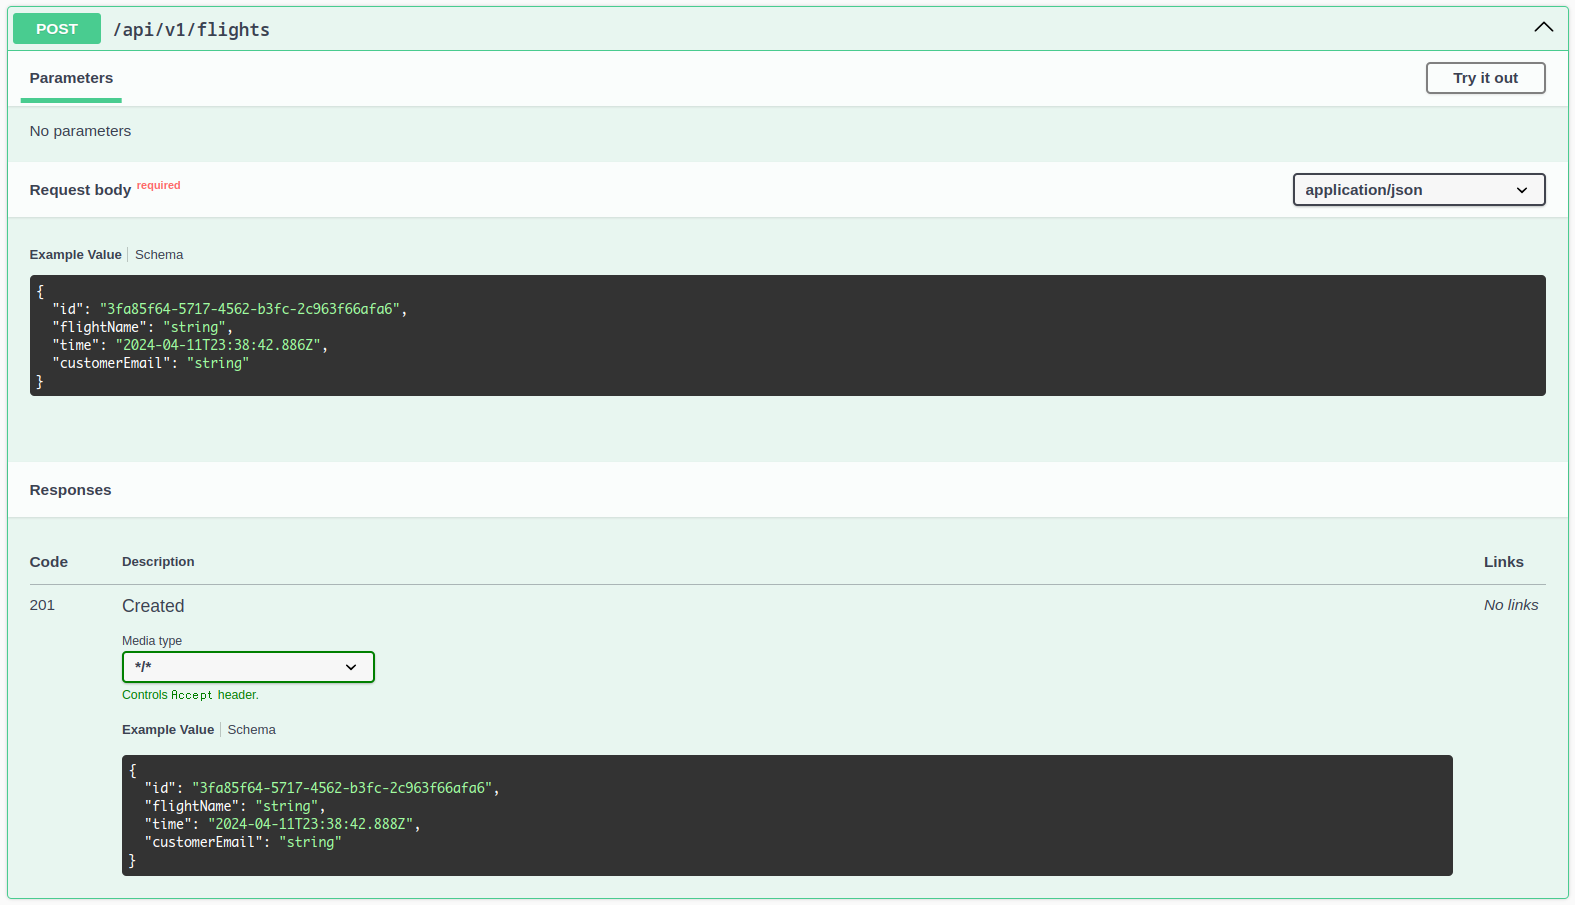
\includegraphics[width=0.8\textwidth, height=0.6\textheight]{img/swagger-doc.png}
		\end{center}		
	
\end{frame}


\begin{frame}[t]{Hypermedia}
		
		User uses APIs according to his understanding with the help of communications support, calling APIs using \textit{resources}. Eventually the user will need to follow some more resources' calls. You might be think of:
		
		\scriptsize		
		\begin{itemize}
			\item<1-> How can the user/client know which request he needs to make next?
			\item<2-> How should the request should look like?
			\item<3-> Which types of error should the client expect?
			
			\item<4->[] \normalsize The answer to this is \textit{"hpermedia"}
			
			\item<5->[] 
				\small
				\begin{block}{Hypermedia}
					Hypermedia is a way for the server to tell the client what HTTP requests the client might want to make in the future. It’s a menu, provided by the server, from which the client is free to choose. The server knows what might happen, but the client decides what actually happens.
				\end{block}
		\end{itemize}		

\tiny source: \href{https://www.oreilly.com/library/view/restful-web-apis/9781449359713/} {\textcolor{blue}{Restful Web APIs}} 	
\end{frame}


\section{API Security}
\begin{frame}{API Security}
  \begin{itemize}
    \item Authentication and Authorization Mechanisms (OAuth, JWT)
    \item Securing API Endpoints
    \item Handling Sensitive Data and Privacy Concerns
  \end{itemize}
\end{frame}

\section{API Testing and Quality Assurance}
\begin{frame}{API Testing and Quality Assurance}
  \begin{itemize}
    \item Writing Effective API Tests
    \item Tools and Frameworks for API Testing
    \item Performance Testing and Load Testing for APIs
  \end{itemize}
\end{frame}


\section{API Management and Lifecycle}
\begin{frame}{API Management and Lifecycle}
  \begin{itemize}
    \item The Lifecycle of API Development
    \item API Deployment Strategies
    \item Monitoring and Analytics for APIs
  \end{itemize}
\end{frame}

\section{Conclusion}
\begin{frame}{Conclusion}
  \begin{itemize}
    \item Recap of Key Learnings
    \item Emerging Trends in API Development
  \end{itemize}
\end{frame}

\end{document}
